% Copyright 2026  Ed Bueler

\documentclass[10pt,
               svgnames,
               hyperref={colorlinks,
                         citecolor=DeepPink4,
                         linkcolor=FireBrick,
                         urlcolor=Maroon},
               usepdftitle=false]{beamer}

\usetheme{Madrid}
\usecolortheme{beaver}
\setbeamercovered{transparent}
\setbeamerfont{frametitle}{size=\large}
\setbeamercolor*{block title}{bg=red!10}
\setbeamercolor*{block body}{bg=red!5}

\usepackage[english]{babel}
\usepackage[latin1]{inputenc}
\usepackage{times}
\usepackage[T1]{fontenc}
% Or whatever. Note that the encoding and the font should match. If T1
% does not look nice, try deleting the line with the fontenc.

\usepackage{fancyvrb,empheq,bm,xspace,dsfont}
%\usepackage{minted}
%\usepackage{hyperref}
\usepackage{tikz}

% If you wish to uncover everything in a step-wise fashion, uncomment
% the following command: 
%\beamerdefaultoverlayspecification{<+->}

\newcommand{\bb}{\mathbf{b}}
\newcommand{\bc}{\mathbf{c}}
\newcommand{\bbf}{\mathbf{f}}
\newcommand{\bl}{\bm{\ell}}
\newcommand{\br}{\mathbf{r}}
\newcommand{\bs}{\mathbf{s}}
\newcommand{\bx}{\mathbf{x}}
\newcommand{\by}{\mathbf{y}}
\newcommand{\bv}{\mathbf{v}}
\newcommand{\bu}{\mathbf{u}}
\newcommand{\bw}{\mathbf{w}}

\newcommand{\bzero}{\bm{0}}

\newcommand{\CC}{\mathbb{C}}
\newcommand{\NN}{\mathbb{N}}
\newcommand{\RR}{\mathbb{R}}
\newcommand{\ZZ}{\mathbb{Z}}

\newcommand{\one}{\mathds{1}}

\newcommand{\range}{\operatorname{range}}
\newcommand{\Span}{\operatorname{span}}

\newcommand{\ddt}[1]{\ensuremath{\frac{\partial #1}{\partial t}}}
\newcommand{\ddx}[1]{\ensuremath{\frac{\partial #1}{\partial x}}}

\newcommand{\Matlab}{\textsc{Matlab}\xspace}
\newcommand{\eps}{\epsilon}

\newcommand{\ds}{\displaystyle}

\newcommand{\ip}[2]{\left<#1,#2\right>}

\newcommand{\twovect}[4]{\ensuremath{{#1}_{#2} =
                            \begin{bmatrix} #3 \\ #4 \end{bmatrix}}}

\newcommand{\rbullet}{{\color{FireBrick} \bullet}}

\newcommand*\circled[1]{\tikz[baseline=(char.base)]{
            \node[shape=circle,draw,inner sep=2pt] (char) {#1};}}

\newcommand{\textbook}{Saxe, \emph{Beginning Functional Analysis}}

\DefineVerbatimEnvironment{mVerb}{Verbatim}{numbersep=2mm,
frame=lines,framerule=0.1mm,framesep=2mm,xleftmargin=4mm,fontsize=\scriptsize}



\title{Fourier series for a continuous function}

\subtitle{a calculation for week 4}

\author{Ed Bueler}

\institute[]{UAF Math 617 Functional Analysis}

\date{Spring 2026}


\begin{document}
\beamertemplatenavigationsymbolsempty

\begin{frame}
  \maketitle
\end{frame}


\begin{frame}{Outline}
  \tableofcontents[hideallsubsections]
\end{frame}

\AtBeginSection[]
{% do not put toc here this time
}


\section{sines (and complex exponentials) are orthonormal}

\begin{frame}{product of sines integral}

\begin{itemize}
\item for $n\in\NN$, $\sin(nx)$ is a \emph{wave} on $[0,\pi]$
\item suppose $m,n\in\NN$ and integrate the product of sines:
\end{itemize}
\begin{align*}
\int_0^\pi \sin(mx)\sin(nx)\,dx &= \hspace{50mm} \\
&\phantom{foo} \\
&\phantom{foo} \\
&\phantom{foo} \\
&\phantom{foo} \\
&\phantom{foo} \\
&\phantom{foo} \\
  &\hspace{50mm} = \begin{cases} \frac{\pi}{2}, & m=n \\ 0, & \text{otherwise} \end{cases}
\end{align*}

\noindent \hrulefill

\noindent {\small \alert{$\cos(\theta \pm \psi) = \cos \theta \cos \psi \mp \sin \theta \sin \psi$} \, $\therefore$ \, $\sin \theta \sin \psi = \frac{1}{2} \left(\cos(\theta-\psi) - \cos(\theta + \psi)\right)$}
\end{frame}


\begin{frame}{an infinite orthonormal set in $C[0,\pi]$}

\begin{itemize}
\item fact from last slide: \quad $\ds \int_0^\pi \sin(mx)\sin(nx)\,dx = \frac{\pi}{2} \delta_{mn}$
\item define
    $$\phi_n(x) = \sqrt{\frac{2}{\pi}} \sin(n x) \qquad \text{and} \qquad S = \left\{\phi_n(x)\,:\,n\in \NN\right\}$$
\item then:
    \begin{enumerate}
    \item $S$ is orthonormal in the (real) inner product $\ip{f}{g} = \int_0^{\pi} f(x)g(x)\,dx$:

\vspace{15mm}
    \item $S$ is linearly independent:

\vspace{15mm}
    \end{enumerate}
\item \emph{questions:}  what is $\Span(S)$?  what is $\overline{\Span(S)}$?
\end{itemize}
\end{frame}


\begin{frame}{an infinite orthonormal set in $C[0,\pi]$}

\begin{center}
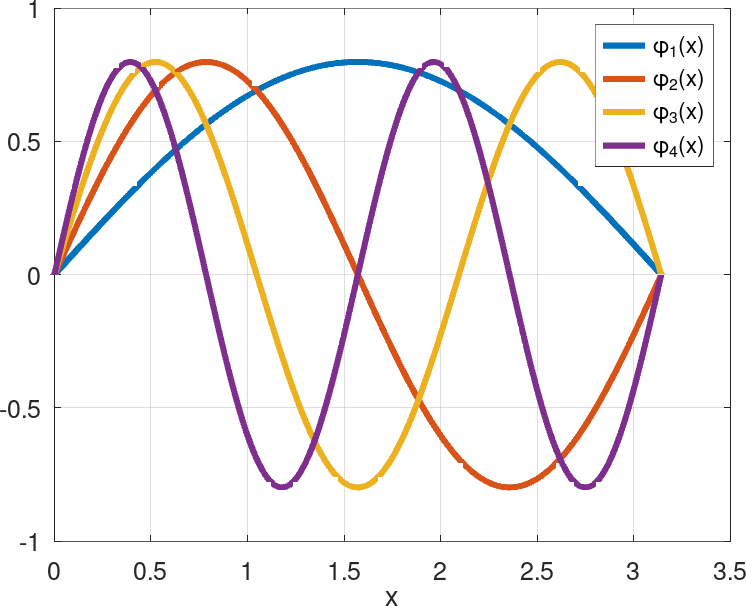
\includegraphics[width=0.8\textwidth]{figs/fourier1sines.png}
\end{center}
\end{frame}


\begin{frame}{a complex-valued orthonormal set in $C[-\pi,\pi]$}

\begin{itemize}
\item \emph{easier} integral:
	$$\int_{-\pi}^\pi e^{imx} e^{-inx}\,dx = \int_{-\pi}^\pi e^{i(m-n)x}\,dx = \hspace{40mm} = 2\pi \delta_{mn}$$
\item define
    $$\psi_n(x) = \frac{1}{\sqrt{2\pi}} e^{inx} \qquad \text{and} \qquad E = \left\{\psi_n(x)\,:\,n\in \ZZ\right\}$$
\item recall \emph{complex} inner product (\emph{sesquilinear}), now on $C[-\pi,\pi]$:
	$$\ip{f}{g} = \int_{-\pi}^\pi f(x) \overline{g(x)}\,dx$$
\item then:
    \begin{enumerate}
    \item $E$ is orthonormal
    \item $E$ is linearly-independent
    \end{enumerate}
\item same \emph{questions:}  what is $\Span(E)$?  what is $\overline{\Span(E)}$?
\end{itemize}
\end{frame}


\AtBeginSection[] {
    \begin{frame}{Outline}
    \setbeamertemplate{section in toc}[sections numbered]
    \tableofcontents[currentsection]%,hideallsubsections]
    \end{frame}
}


\section{what did Fourier believe? (1822)}

\begin{frame}{Fourier's assertion}

\begin{block}{claim (Fourier, \emph{Th\'eorie Analytique de la Chaleur}, 1822)}
if $f\in C[0,\pi]$, and if we compute these coefficients
	$$c_n = \ip{f}{\phi_n} = \sqrt{\frac{2}{\pi}} \int_0^\pi f(x) \sin(nx)\,dx$$
for $n\in \NN$, then
	$$f(x) \stackrel{\ast}{=} \sum_{n=1}^\infty c_n\, \phi_n(x) = \sqrt{\frac{2}{\pi}} \sum_{n=1}^\infty c_n \sin(nx)$$
\end{block}

\begin{itemize}
\item the right side of $\ast$ is the \emph{Fourier sine series} (or \emph{expansion}) of $f$
\item actually Fourier claimed this for discontinuous functions too
   \begin{itemize}
   \item[$\circ$] he, and everybody else, agreed that the claim could not be exactly true at points of discontinuity
   \item[$\circ$] $c_n$ is an \emph{integral}, so only those features of $f$ that change the integrals can affect the expansion
   \end{itemize}
\end{itemize}
\end{frame}


\begin{frame}{complex version}

\begin{itemize}
\item Fourier used real numbers (to my knowledge)
\item we may replace:
	$$C[0,\pi] \to C[-\pi,\pi] \qquad \text{and} \qquad \sin(nx) \to e^{inx},$$
\item we must also make the inner product complex
\end{itemize}

\begin{block}{essential claim}
if $f\in C[-\pi,\pi]$, complex-valued, and if
	$$c_n = \ip{f}{\psi_n} = \frac{1}{\sqrt{2\pi}} \int_{-\pi}^\pi f(x) e^{-inx}\,dx$$
for $n\in\ZZ$, then
	$$f(x) \stackrel{\ast}{=} \sum_{n\in\ZZ} c_n\, \psi_n(x) = \frac{1}{\sqrt{2\pi}} \sum_{n\in\ZZ} c_n e^{inx}$$
\end{block}

\begin{itemize}
\item called the \emph{Fourier series} of $f$, or the \emph{complex Fourier series}
\item for formulas from different references, be careful with where the $2\pi$ goes
\end{itemize}
\end{frame}


\begin{frame}{example 1: $f(x)=x$}

\begin{itemize}
\item we check Fourier's claim for $f(x)=x \in C[0,\pi]$
\item using the real orthonormal set $\left\{\phi_n(x) = \sqrt{\frac{2}{\pi}} \sin(n x)\right\} \subset C[0,\pi]$
\item integrate to get coefficients:
\begin{align*}
c_n &= \ip{f}{\phi_n} = \sqrt{\frac{2}{\pi}} \int_0^\pi x \sin(n x)\,dx = \hspace{60mm} \\
&\phantom{x} \\
&\phantom{x} \\
&\phantom{x} \\
&\phantom{x} \\
&\phantom{x} \hspace{80mm} = \frac{\sqrt{2\pi} (-1)^{n-1}}{n}
\end{align*}
\end{itemize}
\end{frame}


\begin{frame}[fragile]
\frametitle{example 1: $f(x)=x$}

\begin{itemize}
\item \Matlab:
\begin{mVerb}
f = @(x) x;
x = 0:pi/300:pi;
N = 150;  nn = 1:N;
c = sqrt(2 * pi) * (-1).^(nn - 1) ./ nn;
sN = zeros(size(x));
for n=1:N
    sN = sN + c(n) * sqrt(2/pi) * sin(n*x);
end
plot(x, f(x), x, sN)
\end{mVerb}
\item result (works \dots but \emph{Gibbs effect}!):

\begin{center}
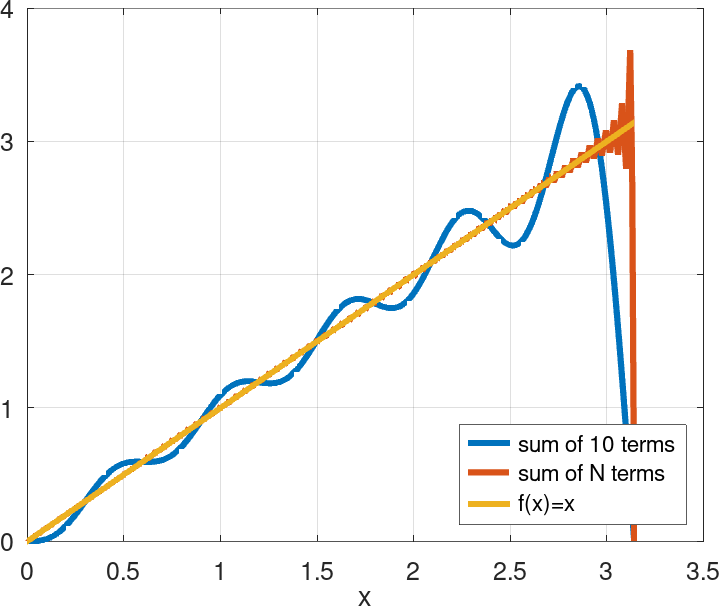
\includegraphics[width=0.4\textwidth]{figs/fourier1result.png}
\end{center}
\end{itemize}
\end{frame}


\begin{frame}{example 2: $g(x)$ cubic}

\begin{itemize}
\item note that if $f(x)=x$ is extended periodically to the real line then the result is \emph{not} continuous
\item let $g(x) = x (x-1) (x-\pi)$ on the interval $[0,\pi]$
\item now the periodic extension \emph{is} continuous
\item coefficients: \quad $\ds c_n = \ip{g}{\phi_n} = \sqrt{\frac{2}{\pi}} \int_0^\pi g(x) \sin(n x)\,dx$
\item but we do these integrals numerically \dots
\end{itemize}

\noindent \alert{\hrulefill}

\begin{columns}
\begin{column}{0.5\textwidth}
\Matlab result:

\begin{center}
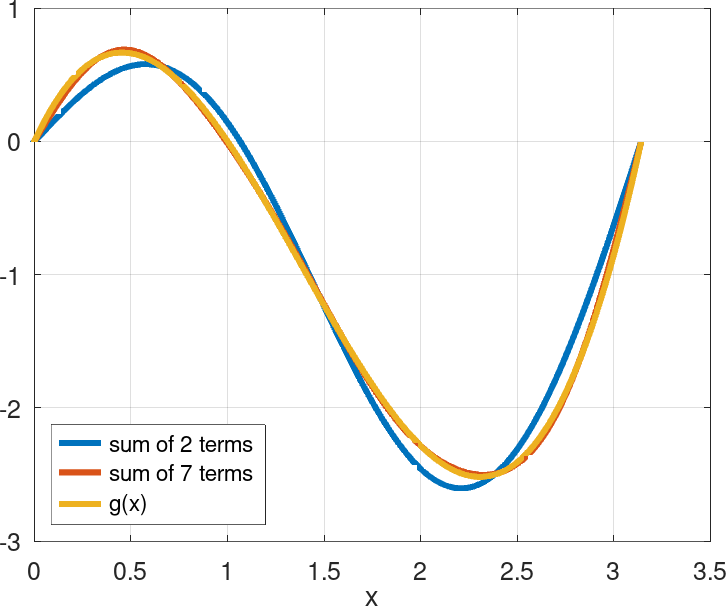
\includegraphics[width=0.7\textwidth]{figs/fourier2result.png}
\end{center}
\end{column}
\begin{column}{0.5\textwidth}
coefficient decay:

\begin{center}
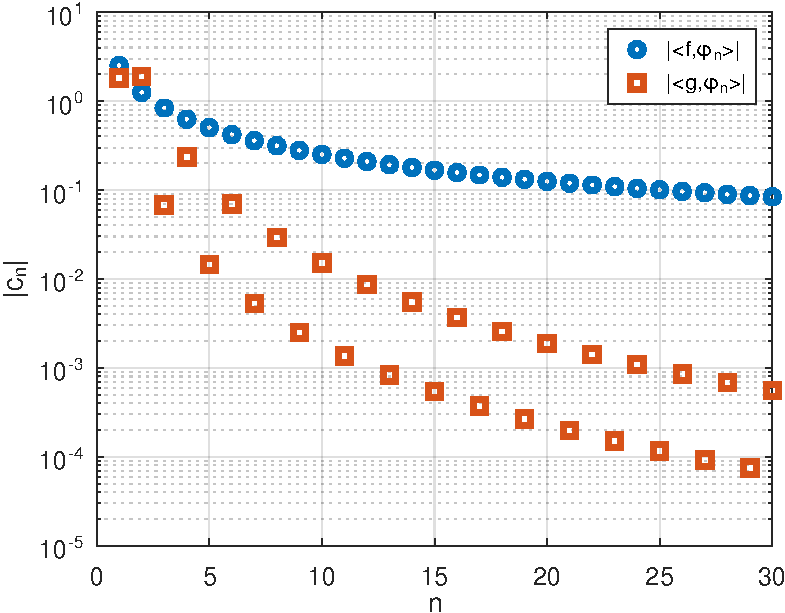
\includegraphics[width=0.8\textwidth]{figs/coeffs12result.pdf}
\end{center}
\end{column}
\end{columns}
\end{frame}


\section{what did Dirichlet prove? (1829)}

\begin{frame}{x}

\begin{block}{y}
x
\end{block}

\begin{itemize}
\item z
\end{itemize}
\end{frame}




\section{what is actually true? (1964)}

\begin{frame}{x}

\begin{block}{y}
x
\end{block}

\begin{itemize}
\item z
\end{itemize}
\end{frame}


\section{what was Hilbert's version? ($\sim$1910)}

\begin{frame}{x}

\begin{block}{y}
x
\end{block}

\begin{itemize}
\item z
\end{itemize}
\end{frame}


\section{theory from the book}

\begin{frame}{theory in week 4: Chapter 4 in Saxe}

FIXME do I want to put Fourier series stuff before measure theory?

\begin{block}{to define:}
\begin{itemize}
\item x
\end{itemize}
\end{block}

\begin{block}{to prove:}
\begin{itemize}
\item Y theorem
\end{itemize}
\end{block}

\begin{itemize}
\item Assignment 3 is posted at \quad  \href{https://bueler.github.io/fa/index.html}{\texttt{bueler.github.io/fa}}
\end{itemize}
\end{frame}


\end{document}
